\let\negmedspace\undefined
\let\negthickspace\undefined
\documentclass[journal]{IEEEtran}
\usepackage[a4paper, margin=10mm, onecolumn]{geometry}
%\usepackage{lmodern} % Ensure lmodern is loaded for pdflatex
\usepackage{tfrupee} % Include tfrupee package

\setlength{\headheight}{1cm} % Set the height of the header box
\setlength{\headsep}{0mm}  % Set the distance between the header box and the top of the text

\usepackage{gvv-book}
\usepackage{gvv}
\usepackage{cite}
\usepackage{amsmath,amssymb,amsfonts,amsthm}
\usepackage{algorithmic}
\usepackage{graphicx}
\usepackage{float}
\usepackage{textcomp}
\usepackage{xcolor}
\usepackage{txfonts}
\usepackage{listings}
\usepackage{enumitem}
\usepackage{mathtools}
\usepackage{gensymb}
\usepackage{comment}
\usepackage[breaklinks=true]{hyperref}
\usepackage{tkz-euclide} 
\usepackage{listings}
% \usepackage{gvv}                                        
\def\inputGnumericTable{}                                 
\usepackage[latin1]{inputenc}                                
\usepackage{color}                                            
\usepackage{array}                                            
\usepackage{longtable}                                       
\usepackage{calc}                                             
\usepackage{multirow}                                         
\usepackage{hhline}                                           
\usepackage{ifthen}                                           
\usepackage{lscape}
\usepackage{tikz}
\usetikzlibrary{patterns}

\begin{document}

\bibliographystyle{IEEEtran}
\vspace{3cm}

\title{GATE-04}
\author{ee25btech11063-vejith}

\maketitle
% \maketitle
% \newpage
% \bigskip
{\let\newpage\relax\maketitle}
\renewcommand{\thefigure}{\theenumi}
\renewcommand{\thetable}{\theenumi}
\setlength{\intextsep}{10pt} % Space between text and floats
\begin{enumerate}[start=1]
\item Inhaling the smoke from a burning \underline{\hspace{2cm}} could \underline{\hspace{2cm}} you quickly.

\hfill{\brak{\text{GATE GG 2022}}}
\begin{enumerate}
\item tire/tier
\item tire/tyre
\item tyre/tire
\item tyre/tier
\end{enumerate}

\item A sphere of radius $r$ cm is packed in a box of cubical shape. What should be the minimum volume \brak{\text{in } cm^3} of the box that can enclose the sphere?

\hfill{\brak{\text{GATE GG 2022}}}
\begin{enumerate}
\item $\frac{r^3}{8}$
\item $r^3$
\item $2r^3$
\item $8r^3$
\end{enumerate}

\item Pipes P and Q can fill a storage tank in full with water in $10$ and $6$ minutes, respectively. Pipe R draws the water out from the storage tank at a rate of $34$ litres per minute. P, Q and R operate at a constant rate. If it takes one hour to completely empty a full storage tank with all the pipes operating simultaneously, what is the capacity of the storage tank \brak{\text{in litres}}?

\hfill{\brak{\text{GATE GG 2022}}}
\begin{enumerate}
\item $26.8$
\item $60.0$
\item $120.0$
\item $127.5$
\end{enumerate}

\item Six persons P, Q, R, S, T and U are sitting around a circular table facing the center not necessarily in the same order. Consider the following statements:
\begin{itemize}
\item P sits next to S and T.
\item Q sits diametrically opposite to P.
\item The shortest distance between S and R is equal to the shortest distance between T and U.
\end{itemize}
Based on the above statements, Q is a neighbor of

\hfill{\brak{\text{GATE GG 2022}}}
\begin{enumerate}
\item U and S
\item R and T
\item R and U
\item P and S
\end{enumerate}

\item A building has several rooms and doors as shown in the top view of the building given below. The doors are closed initially. What is the minimum number of doors that need to be opened in order to go from the point P to the point Q?

\hfill{\brak{\text{GATE GG 2022}}}
\begin{figure}[H]
\centering
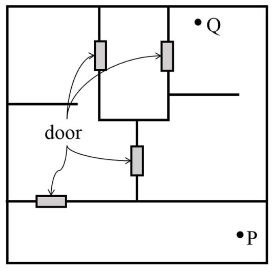
\includegraphics[width = 0.42\columnwidth]{figs/01.png}
\caption*{}
\label{fig:q5}
\end{figure}
\begin{enumerate}
\item $4$
\item $3$
\item $2$
\item $1$
\end{enumerate}

\item Rice, a versatile and inexpensive source of carbohydrate, is a critical component of diet worldwide. Climate change, causing extreme weather, poses a threat to sustained availability of rice. Scientists are working on developing Green Super Rice (GSR), which is resilient under extreme weather conditions yet gives higher yields sustainably. Which one of the following is the CORRECT logical inference based on the information given in the above passage?

\hfill{\brak{\text{GATE GG 2022}}}
\begin{enumerate}
\item GSR is an alternative to regular rice, but it grows only in an extreme weather
\item GSR may be used in future in response to adverse effects of climate change
\item GSR grows in an extreme weather, but the quantity of produce is lesser than regular rice
\item Regular rice will continue to provide good yields even in extreme weather
\end{enumerate}

\item A game consists of spinning an arrow around a stationary disk as shown below. When the arrow comes to rest, there are eight equally likely outcomes. It could come to rest in any one of the sectors numbered $1$, $2$, $3$, $4$, $5$, $6$, $7$ or $8$ as shown. Two such disks are used in a game where their arrows are independently spun. What is the probability that the sum of the numbers on the resulting sectors upon spinning the two disks is equal to $8$ after the arrows come to rest?

\hfill{\brak{\text{GATE GG 2022}}}
\begin{figure}[H]
\centering
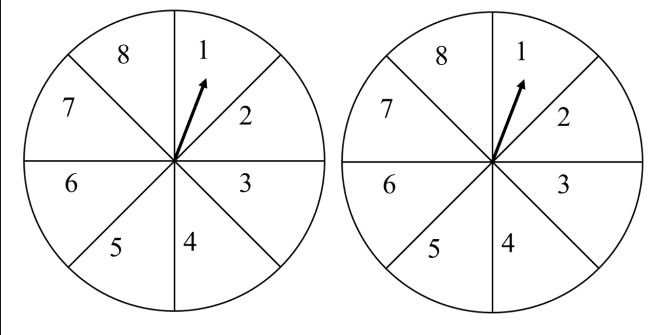
\includegraphics[width = 0.5\columnwidth]{figs/02.png}
\caption*{}
\label{fig:q7}
\end{figure}
\begin{enumerate}
\item $\frac{1}{16}$
\vspace{0.3cm}
\item $\frac{5}{64}$
\vspace{0.3cm}
\item $\frac{3}{32}$
\vspace{0.3cm}
\item $\frac{7}{64}$
\end{enumerate}

\item Consider the following inequalities.
\begin{align*}
\brak{\text{i}} \qquad 3p-q&<4\\
\brak{\text{ii}}\qquad 3q-p&<12
\end{align*}
Which one of the following expressions below satisfies the above two inequalities?

\hfill{\brak{\text{GATE GG 2022}}}
\begin{enumerate}
\item $p+q<8$
\item $p+q=8$
\item $8\le p+q<16$
\item $p+q\ge16$
\end{enumerate}

\item Given below are three statements and four conclusions drawn based on the statements.
\begin{itemize}
\item Statement 1: Some engineers are writers.
\item Statement 2: No writer is an actor.
\item Statement 3: All actors are engineers.
\end{itemize}
\begin{itemize}
\item Conclusion I: Some writers are engineers.
\item Conclusion II: All engineers are actors.
\item Conclusion III: No actor is a writer.
\item Conclusion IV: Some actors are writers.
\end{itemize}
Which one of the following options can be logically inferred?

\hfill{\brak{\text{GATE GG 2022}}}
\begin{enumerate}
\item Only conclusion I is correct
\item Only conclusion II and conclusion III are correct
\item Only conclusion I and conclusion III are correct
\item Either conclusion III or conclusion IV is correct
\end{enumerate}

\item Which one of the following sets of pieces can be assembled to form a square with a single round hole near the center? Pieces cannot overlap.

\hfill{\brak{\text{GATE GG 2022}}}
\begin{figure}[H]
\begin{enumerate}
\item \centering 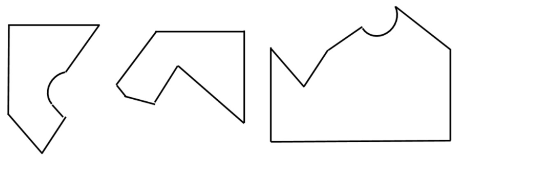
\includegraphics[width = 0.5\columnwidth]{figs/03.png} 
\item \centering 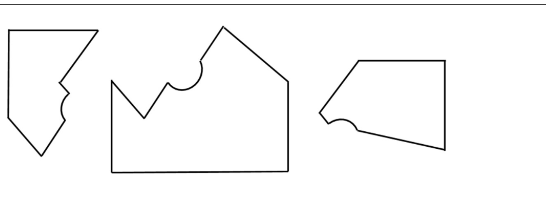
\includegraphics[width = 0.5\columnwidth]{figs/04.png}
\item \centering 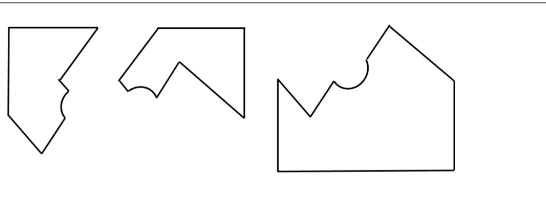
\includegraphics[width = 0.5\columnwidth]{figs/05.png}
\item \centering 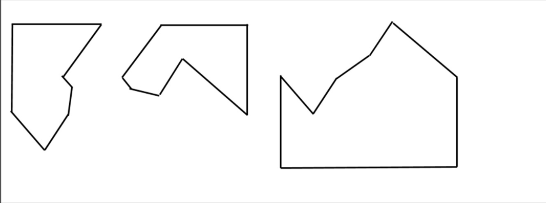
\includegraphics[width = 0.5\columnwidth]{figs/06.png}
\end{enumerate}
\caption*{}
\label{fig:q10}
\end{figure}

\item Which one of the following is the typical product of ductile deformation?

\hfill(GATE GG 2022)
\begin{enumerate}
\item Gouge
\item Breccia
\item Cataclasite
\item Mylonite
\end{enumerate}

\item Which one among the following coastal erosional landforms is caused by the action of sea waves?

\hfill(GATE GG 2022)
\begin{enumerate}
\item Ventifact
\item Kettle
\item Cirque
\item Cliff
\end{enumerate}

\item In which one of the following regions of the electromagnetic spectrum does the maximum atmospheric scattering occur?

\hfill(GATE GG 2022)
\begin{enumerate}
\item UV
\item IR
\item Radiowave
\item Microwave
\end{enumerate}

\item Which one of the following is the Poisson$'$s ratio for an incompressible fluid?

\hfill(GATE GG 2022)
\begin{enumerate}
\item $0$
\item $0.25$
\item $1$
\item $0.5$
\end{enumerate}

 \item Which among the following Period(s) belong(s) to the Paleozoic Era?

\hfill(GATE GG 2022)
\begin{enumerate}
\item Carboniferous
\item Paleogene
\item Silurian
\item Cretaceous
\end{enumerate}
\vspace{0.3cm}

\item The average bulk density of a fully saturated sandstone reservoir with a fractional porosity of $0.23$ is  \makebox[2cm]{\hrulefill} g/cc. \sbrak{\text{round off to $2$ decimal places}} \\
\sbrak{\text{Assume matrix density = $2.63$ g/cc and fluid density = $1.05$ g/cc}}
\hfill(GATE GG 2022)

\vspace{0.5cm}
\item For a productive alluvial aquifer with hydraulic conductivity = $105$ m/day and hydraulic gradient = $0.01$, the flow rate is \makebox[2cm]{\hrulefill} m/day. [round off to $2$ decimal places]
\hfill(GATE GG 2022)
\vspace{0.5cm}

\item The relationship between conjugate shear fractures and the principal stresses in a homogenous, isotropic, deformed body is shown in the stereoplot 
($\sigma_1, \sigma_2, \sigma_3$ are compressive stresses).  Which one of the given fault regimes is indicated according to the Anderson$'$s theory of faulting for the formation of conjugate shear fractures under plane strain?
\hfill(GATE GG 2022)
\begin{figure}[H]
\centering
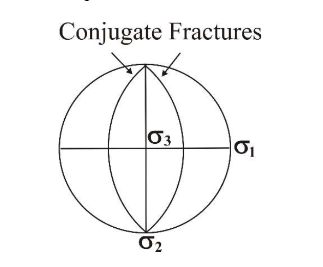
\includegraphics[width = 0.42\columnwidth]{figs/07.png}
\caption*{}
\label{fig:q5}
\end{figure}
\begin{multicols}{2}
\begin{enumerate}
\item Dextral strike-slip
\item Sinistral strike-slip
\item Reverse
\item Normal
\end{enumerate}
\end{multicols}

\item How many independent elastic parameters are needed to describe a homogenous isotropic material?

\hfill(GATE GG 2022)
\begin{enumerate}
\item $21$
\item $2$
\item $36$
\item $3$
\end{enumerate}

\item Which one of the following is a mafic volcanic rock?

\hfill(GATE GG 2022)
\begin{enumerate}
\item Dacite
\item Trachyte
\item Rhyolite
\item Basalt
\end{enumerate}

\item The intercepts of a crystal face on the crystallographic axes are $\infty a, 2b, 3c$.  
Which one of the following is its Miller Index?

\hfill(GATE GG 2022)
\begin{enumerate}
\item (032)
\item (023)
\item (203)
\item (320)
\end{enumerate}

\item Match the locations in Group I with the corresponding economic deposits in Group II.
\hfill(GATE GG 2022)
\begin{tabular}{ l l }
\textbf{Group I} & \textbf{Group Il}\\
P. Wajrakarur & 1. Chromite \\
 Q. Sukinda & 2. Diamond\\
 R. Malanjkhand &  3. Barite\\
 S. Mangampeta & 4. Copper
\end{tabular}
\begin{enumerate}
\item P-3; Q-4; R-1; S-2
\item P-3; Q-1; R-4; S-2
\item P-2; Q-1; R-4; S-3
\item P-2; Q-4; R-1; S-3
\end{enumerate}

\item Choose the CORRECT statement(s) on seismic wave propagation in an elastic isotropic medium.

\hfill(GATE GG 2022)
\begin{enumerate}
\item P-waves are polarized in the direction of propagation
\item S-waves are polarized in the direction of propagation
\item Rayleigh waves are elliptically polarized
\item Love waves are elliptically polarized
\end{enumerate}

\item The difference in arrival times of P- and S-waves generated by an earthquake and recorded at a seismological station is one second. Assuming VP = $3$ km/s and VP/VS = $2.0$, the distance between the station and the hypocenter is \makebox[2cm]{\hrulefill} km. \sbrak{\text{round off to $1$ decimal place}}
\hfill(GATE GG 2022)
\vspace{0.5cm}

\item Assuming the rate of rotation of the Earth is $7.27 \times 10^{-5}$ rad/s and the radius of Earth is $6371$ km, the centrifugal acceleration at $60\degree$ latitude is  \makebox[2cm]{\hrulefill}$\times 10^{-3}$ m/s$^2$. \sbrak{\text{round off to 1 decimal place}}
\hfill(GATE GG 2022)
\vspace{0.5cm}

\item The angle of inclination of the remanent magnetization of a volcanic rock measured at a location is 45$\degree$. The magnetic latitude of the location of the volcanic rock at the time of its magnetization is  \makebox[2cm]{\hrulefill}$\degree$N. \sbrak{\text{round off to 1 decimal place}}\\
\hfill(GATE GG 2022)

\textbf{PART B (SECTION 1):FOR GEOLOGY CANDIDATES ONLY}
\vspace{0.5cm}

\item A coarse-grained igneous rock consists of 55\% olivine, 25\% augite and 20\% 
enstatite. According to the IUGS classification, the rock is  

\hfill(GATE GG 2022)
\begin{enumerate}
\item websterite
\item lherzolite
\item wehrlite
\item harzburgite
\end{enumerate}

\item The rock-type used to build the walls of the Red Fort in Delhi is  

\hfill(GATE GG 2022)
\begin{enumerate}
\item sandstone
\item marble
\item granite
\item basalt
\end{enumerate}

\item During crystallization of a magma, which one of the following schematic paths \brak{I, II, III and IV} describes the behavior of compatible elements in the residual melt?
\hfill(GATE GG 2022)
\begin{figure}[H]
\centering
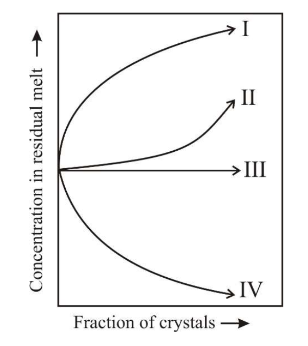
\includegraphics[width = 0.47\columnwidth]{figs/08.png}
\caption*{}
\label{fig:q5}
\end{figure}
\begin{enumerate}
\item II
\item IV
\item I
\item III
\end{enumerate}


\item In the geological map of India, which one of the following geological units has the largest area? 

\hfill(GATE GG 2022)
\begin{enumerate}
\item Vindhyan Supergroup
\item Deccan Volcanic Province
\item Singhbhum Granite
\item Mesozoic rocks of Kutch
\end{enumerate}
\vspace{0.8cm}

\item Which one of the following cross-stratifications provides the paleocurrent direction on the truncated bedding surface of an undeformed cross-stratified sedimentary strata?  

\hfill(GATE GG 2022)
\begin{enumerate}
\item Tabular
\item Hummocky
\item Trough
\item Herringbone
\end{enumerate}
\vspace{0.5cm}

\item Which one of the following is a dinosaur?  

\hfill(GATE GG 2022)
\begin{enumerate}
\item Stegodon
\item Stegosaurus
\item Equus
\item Otoceras
\end{enumerate}
\vspace{0.5cm}

\item The Hoek-Brown failure envelope is typically the segment of which one of the following?  

\hfill(GATE GG 2022)
\begin{enumerate}
\item Straight line
\item Ellipse
\item Parabola
\item Hyperbola
\end{enumerate}
\vspace{0.5cm}


\item Which one of the following is the optical spectral window suitable for remote sensing?  

\hfill(GATE GG 2022)
\begin{enumerate}
\item $0.02$ - $0.2$ $\mu$m
\item $0.4$ - $14$ $\mu$m
\item $0.8$ - $2.0$ $\mu$m
\item $0.01$ - $1$ $\mu$m
\end{enumerate}
\vspace{0.5cm}

\item A radioactive nucleus $X_{92}^{238}$ decays to $Y_{82}^{206}$.  
The number of $\alpha$ and $\beta$ particles emitted during this decay are 

\hfill(GATE GG 2022)
\begin{enumerate}
\item 12$\alpha$ and 1$\beta^{+}$
\item 6$\alpha$ and 1$\beta^{-}$
\item 3$\alpha$ and 1$\beta^{+}$
\item 3$\alpha$ and 1$\beta^{-}$ 
\end{enumerate}
\vspace{0.5cm}


\item The silicate mineral(s) that commonly occur(s) in regionally metamorphosed 
siliceous dolomitic limestone is/are  

\hfill(GATE GG 2022)
\begin{enumerate}
\item diopside
\item cordierite
\item tremolite
\item wollastonite
\end{enumerate}
\vspace{0.5cm}

\item Which of the natural hazard(s) listed below can be caused by Earthquakes? 

\hfill(GATE GG 2022)
\begin{enumerate}
\item Tsunamis
\item Landslides
\item Cyclones
\item Lightning
\end{enumerate}
\vspace{0.5cm}

\item Which of the following is/are the driving force(s) behind plate motion? 

\hfill(GATE GG 2022)
\begin{enumerate}
\item Slab-Pull
\item Ridge-Push
\item Mantle Convection
\item Advection
\end{enumerate}
\vspace{0.5cm}

\item Which of the following is/are copper ore mineral(s)?  

\hfill(GATE GG 2022)
\begin{enumerate}
\item Bornite
\item Pentlandite
\item Gahnite
\item Covellite
\end{enumerate}
\vspace{0.5cm}

\item Which of the following stratigraphic unit(s) of the Vindhyan Supergroup contain(s) commercially significant limestone deposit(s)?  

\hfill(GATE GG 2022)
\begin{enumerate}
\item Bhander Formation
\item Rewa Formation
\item Kaimur Formation
\item Rohtas Formation
\end{enumerate}
\vspace{0.5cm}

\item The strike and dip of the axial plane of a reclined fold is $02\degree$ and $28\degree$ SE, respectively. The plunge direction (whole circle bearing) of the axis of the reclined fold is\makebox[2cm]{\hrulefill} degrees. \sbrak{\text{In integer}}
\hfill(GATE GG 2022)
\vspace{0.5cm}

\item If the shrinkage factor of a crude oil is $0.7$, its formation volume factor is \makebox[2cm]{\hrulefill}. \sbrak{\text{round off to 1 decimal place}}
\hfill(GATE GG 2022)
\vspace{0.5cm}

\item The cross section of a river channel is approximated by a trapezium. The river has  average width $= 40$ m and average depth $= 3$ m. If the average flow speed is $2$ m/s,  the discharge rate is \makebox[2cm]{\hrulefill} m$^3$/s. \sbrak{\text{In integer}}
\hfill(GATE GG 2022)
\vspace{0.5cm}

\item A mineral of uniform composition is cut into a wedge shape.  
The birefringence of the wedge section is $0.012$. The retardation at $40$ $\mu$m thickness of the wedge is \makebox[2cm]{\hrulefill} nm. \sbrak{\text{integer}}
\hfill(GATE GG 2022)
\vspace{0.5cm}

\item The sand supply and the variability of wind direction results in different dune types. In the options below, choose the CORRECT pair of dune types marked I and II in the figure.
\hfill(GATE GG 2022)
\begin{figure}[H]
\centering
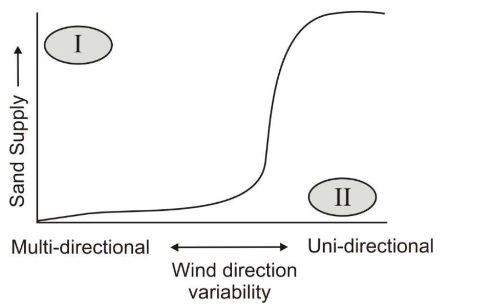
\includegraphics[width = 0.47\columnwidth]{figs/09.png}
\caption*{}
\label{fig:q5}
\end{figure}
\begin{enumerate}
\item I - Transverse dune; II - Barchan dune  
\item I - Star dune; II - Barchan dune  
\item I - Barchan dune; II - Linear dune  
\item I - Barchan dune; II - Star dune  
\end{enumerate}

\item Which one of the following statements is CORRECT?  

\hfill(GATE GG 2022)
\begin{enumerate}
\item Salt dome traps are abundant in the Upper Assam Basin  
\item Fold and thrust related traps are common in the Mumbai Offshore Basin  
\item Limestone is the predominant reservoir rock in the Cambay Basin  
\item Sandstone is the reservoir rock in the Krishna-Godavari Basin  
\end{enumerate}


\item Identify the common metamorphic minerals labelled X and Y in the ACF diagram.  

\hfill(GATE GG 2022)
\begin{figure}[H]
\centering
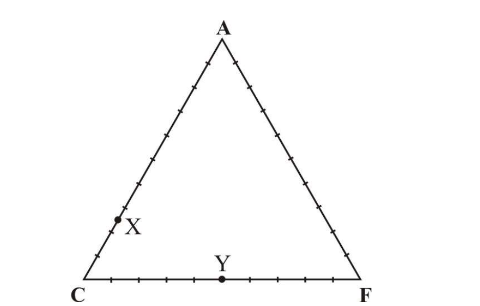
\includegraphics[width = 0.47\columnwidth]{figs/10.png}
\caption*{}
\label{fig:q5}
\end{figure}
\begin{enumerate}
\item X - Anorthite; Y - Actinolite  
\item X - Grossular; Y - Diopside  
\item X - Wollastonite; Y - Almandine  
\item X - Ferrosilite; Y - Andradite  
\end{enumerate}


\item Which one of the following schematic P-T paths is characteristic for a rock metamorphosed in a subduction zone?  

\hfill(GATE GG 2022)
\begin{figure}[H]
\begin{enumerate}
\item \centering 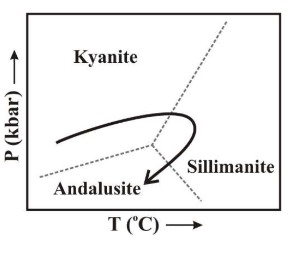
\includegraphics[width = 0.22\columnwidth]{figs/11.png} 
\item \centering 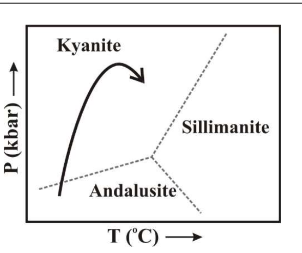
\includegraphics[width = 0.22\columnwidth]{figs/12.png}
\item \centering 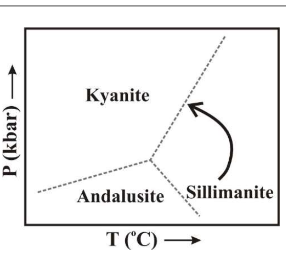
\includegraphics[width = 0.22\columnwidth]{figs/13.png}
\item \centering 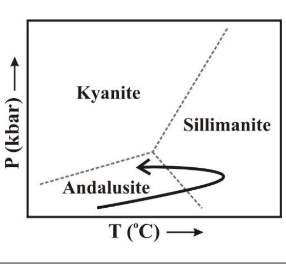
\includegraphics[width = 0.22\columnwidth]{figs/14.png}
\end{enumerate}
\caption*{}
\label{fig:q10}
\end{figure}


\item Which one of the following is the CORRECT statement regarding the ecology of bivalves?  

\hfill(GATE GG 2022)
\begin{enumerate}
\item Pholas is a swimming form  
\item Venus is a shallow burrower  
\item Pecten is a stone borer  
\item Spondylus is a deep burrower  
\end{enumerate}

\item On a fault surface with strike and dip 320$\degree$ and 55$\degree$ NE, respectively, four sets of slickenlines were measured. The plunge and plunge direction of the lineation is  

\hfill(GATE GG 2022)
\begin{enumerate}
\item 55$\degree$ $\to$ 050$\degree$  
\item 20$\degree$ $\to$ 320$\degree$  
\item 50$\degree$ $\to$ 325$\degree$  
\item 60$\degree$ $\to$ 090$\degree$    
\end{enumerate}


\item Match the following tectonic settings in Group-I with the corresponding examples in Group-II. 
\hfill(GATE GG 2022)
\begin{tabular}{ l l}
Group I & Group II \\ 
P. Rift Basin & 1. Pacific Ocean \\
Q. Passive Margin & 2. Gulf of Suez \\
R. Subducting Ocean & 3. West coast of India \\
S. Collision & 4. Mediterranean Sea 
\end{tabular}
\begin{enumerate}
\item P-2; Q-3; R-1; S-4  
\item P-3; Q-2; R-4; S-1  
\item P-2; Q-1; R-3; S-4  
\item P-4; Q-3; R-1; S-2  
\end{enumerate}


\item Match the following igneous textures in Group-I with their definitions in Group-II.  
\hfill(GATE GG 2022)
\begin{tabular}{ l l}
Group I & Group II \\
P. Vitrophyre & 1. Alkali feldspar rimmed by plagioclase \\
Q. Rapakivi & 2. Radial needle-like plagioclase with or without clinopyroxene \\
R. Ocelli & 3. Sub-parallel skeletal, platy olivine/pyroxene \\
S. Spinifex & 4. Large phenocrysts within a glassy matrix \\
\end{tabular}
\begin{enumerate}
\item P-2; Q-3; R-4; S-1  
\item P-3; Q-4; R-2; S-1  
\item P-4; Q-1; R-2; S-3  
\item P-4; Q-1; R-3; S-2 
\end{enumerate}

\item Match the Volcanogenic Massive Sulfide (VMS)-type deposits in Group-I with host rocks in Group-II.  
\hfill(GATE GG 2022)
\begin{tabular}{ l l}
Group I & Group II \\ 
P. Besshi & 1. Felsic volcanics \\
Q. Bathurst & 2. Mafic volcanics + siliciclastics \\
R. Kuroko & 3. Mafic volcanics \\
S. Cyprus & 4. Felsic volcanics + siliciclastics 
\end{tabular}
\begin{enumerate}
\item P-2; Q-1; R-3; S-4  
\item P-2; Q-4; R-1; S-3  
\item P-4; Q-3; R-1; S-2  
\item P-1; Q-4; R-2; S-3  
\end{enumerate}


\item The phase relations diagram (A-B system) shows cooling and crystallization path. Which statements are CORRECT?  

\hfill(GATE GG 2022)
\begin{figure}[H]
\centering
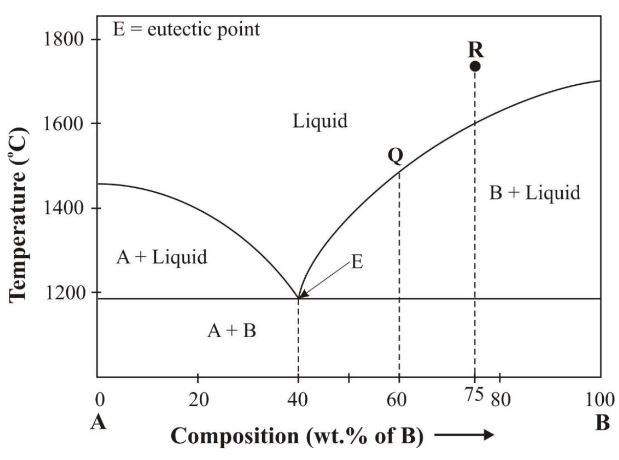
\includegraphics[width = 0.47\columnwidth]{figs/15.png}
\caption*{}
\label{fig:q5}
\end{figure}
\begin{enumerate}
\item On complete crystallization of magma, the final composition (in wt.\%) of rock consists of 25 of mineral A and 75 of mineral B. 
\item On cooling of magma, mineral A is the first mineral to crystallize. 
\item At point Q, the weight percentages of crystal and liquid are 37.5 and 62.5,respectively. 
\item The composition (in wt.\%) of liquid at point E is 40 A and 60 B.
\end{enumerate}

\item Which of the following systems tract(s) indicate regression?  

\hfill(GATE GG 2022)
\begin{enumerate}
\item Transgressive systems tract  
\item Falling stage systems tract  
\item Highstand systems tract  
\item Lowstand systems tract  
\end{enumerate}


\item Which of the following sedimentary feature(s) indicate(s) sub-aerial exposure?  

\hfill(GATE GG 2022)
\begin{enumerate}
\item Groove cast  
\item Double mud drape  
\item Rain print  
\item Adhesion ripple  
\end{enumerate}

\item Which of the following statement(s) is/are correct?  

\hfill(GATE GG 2022)
\begin{enumerate}
\item Diatoms are algal forms  
\item Dinoflagellates are unicellular algae  
\item Petropods are planktic gastropods  
\item Radiolarians are organic-walled microfossils  
\end{enumerate}

\item Which among the following space groups is/are non-compatible with glide plane?  

\hfill(GATE GG 2022)
\begin{enumerate}
\item Pab21  
\item Pnma  
\item P6$_3$/c  
\item P3c1  
\end{enumerate}

\item Which type of porphyroclast(s) are suitable kinematic indicators in ductile shear zones?  

\hfill(GATE GG 2022)
\begin{enumerate}
\item $\sigma$-type  
\item $\Theta$-type  
\item $\delta$-type  
\item $\varphi$-type  
\end{enumerate}

\item Which of the following parameter(s) is/are Rock Mass Rating (RMR) based on?

\hfill(GATE GG 2022)
\begin{enumerate}
\item Rock Quality Designation (RQD)  
\item UCS of intact rock  
\item Groundwater conditions  
\item Rock composition  
\end{enumerate}

\item A sample of $10$ g coal yields $1$ g moisture, $2$ g ash and $5.6$ g volatile matter.  The percentage of volatile matter on dry ash-free basis is \makebox[2cm]{\hrulefill}.\sbrak{\text{round off to 1 decimal place}}  
\hfill(GATE GG 2022)
\vspace{0.5cm}

\item A soil sample shows average beta count of $6.8$ counts per minute \brak{cpm} per gram of organic carbon.The $^{14}$C count rate from organic carbon of  Present-day vegetation = 15.26 cpm/g.  The age of sample is $=$  \makebox[2cm]{\hrulefill}years.(Half-life of $^{14}$C = $5370$ y).\sbrak{\text{round off to 1 decimal place}} 
\hfill(GATE GG 2022)
\vspace{0.5cm}

\item A digital camera with focal length $150$ mm is flown at height $3000$ m.  
The scale of aerial photograph = 1:\makebox[2cm]{\hrulefill}.\sbrak{\text{in integer}}
\hfill(GATE GG 2022)
\vspace{0.5cm}


\item The following reaction occurs at 1 bar and 823 K. \\ 
$\text{Grossular} + \text{Quartz}   = \text{Anorthite} + \text{Wollastonite}$
\begin{table}[h]
    \centering
    \begin{center}
\begin{tabular}{ll}
    \textbf{Group I} & \textbf{Group II} \\
    P. Ferrite & 1. Hexagonal Close Packed (HCP) \\
    Q. Austenite & 2. Body Centered Cubic (BCC) \\
    R. Martensite & 3. Body Centered Tetragonal (BCT) \\
    & 4. Face Centered Cubic (FCC)
\end{tabular}
\end{center}
    \caption{Given Values}
    \label{tab:1}
\end{table}
Using the above molar thermodynamic data, the calculated slope of the above 
reaction is \makebox[2cm]{\hrulefill} bar K$^{-1}$. \sbrak{\text{round off to 2 decimal places}}
\hfill(GATE GG 2022)
\vspace{0.5cm}

\item Operating costs of an open cast gold mine are Rs.$4000$/tonne.  The recovery at the mill is $90$\%. At a gold price of Rs. $4550$/g, the cutoff grade of gold calculated on the basis of operating cost is \makebox[2cm]{\hrulefill}g/tonne. \sbrak{\text{round off to second decimal place}}
\hfill(GATE GG 2022)
\end{enumerate}

\vspace{1cm}
\textbf{SESSSION 2}
\begin{enumerate}
\item Inhaling the smoke from a burning \underline{\hspace{2cm}} could \underline{\hspace{2cm}} you quickly.

\hfill{\brak{\text{GATE GG 2022}}}
\begin{enumerate}
\item tire/tier
\item tire/tyre
\item tyre/tire
\item tyre/tier
\end{enumerate}

\item A sphere of radius $r$ cm is packed in a box of cubical shape. What should be the minimum volume \brak{\text{in } cm^3} of the box that can enclose the sphere?

\hfill{\brak{\text{GATE GG 2022}}}
\begin{enumerate}
\item $\frac{r^3}{8}$
\item $r^3$
\item $2r^3$
\item $8r^3$
\end{enumerate}

\item Pipes P and Q can fill a storage tank in full with water in $10$ and $6$ minutes, respectively. Pipe R draws the water out from the storage tank at a rate of $34$ litres per minute. P, Q and R operate at a constant rate. If it takes one hour to completely empty a full storage tank with all the pipes operating simultaneously, what is the capacity of the storage tank \brak{\text{in litres}}?

\hfill{\brak{\text{GATE GG 2022}}}
\begin{enumerate}
\item $26.8$
\item $60.0$
\item $120.0$
\item $127.5$
\end{enumerate}

\item Six persons P, Q, R, S, T and U are sitting around a circular table facing the center not necessarily in the same order. Consider the following statements:
\begin{itemize}
\item P sits next to S and T.
\item Q sits diametrically opposite to P.
\item The shortest distance between S and R is equal to the shortest distance between T and U.
\end{itemize}
Based on the above statements, Q is a neighbor of

\hfill{\brak{\text{GATE GG 2022}}}
\begin{enumerate}
\item U and S
\item R and T
\item R and U
\item P and S
\end{enumerate}

\item A building has several rooms and doors as shown in the top view of the building given below. The doors are closed initially. What is the minimum number of doors that need to be opened in order to go from the point P to the point Q?

\hfill{\brak{\text{GATE GG 2022}}}
\begin{figure}[H]
\centering
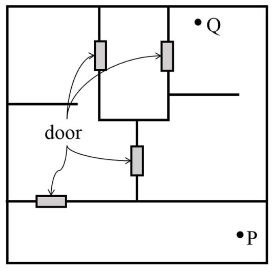
\includegraphics[width = 0.42\columnwidth]{figs/01.png}
\caption*{}
\label{fig:q5}
\end{figure}
\begin{enumerate}
\item $4$
\item $3$
\item $2$
\item $1$
\end{enumerate}

\item Rice, a versatile and inexpensive source of carbohydrate, is a critical component of diet worldwide. Climate change, causing extreme weather, poses a threat to sustained availability of rice. Scientists are working on developing Green Super Rice (GSR), which is resilient under extreme weather conditions yet gives higher yields sustainably. Which one of the following is the CORRECT logical inference based on the information given in the above passage?

\hfill{\brak{\text{GATE GG 2022}}}
\begin{enumerate}
\item GSR is an alternative to regular rice, but it grows only in an extreme weather
\item GSR may be used in future in response to adverse effects of climate change
\item GSR grows in an extreme weather, but the quantity of produce is lesser than regular rice
\item Regular rice will continue to provide good yields even in extreme weather
\end{enumerate}

\item A game consists of spinning an arrow around a stationary disk as shown below. When the arrow comes to rest, there are eight equally likely outcomes. It could come to rest in any one of the sectors numbered $1$, $2$, $3$, $4$, $5$, $6$, $7$ or $8$ as shown. Two such disks are used in a game where their arrows are independently spun. What is the probability that the sum of the numbers on the resulting sectors upon spinning the two disks is equal to $8$ after the arrows come to rest?

\hfill{\brak{\text{GATE GG 2022}}}
\begin{figure}[H]
\centering
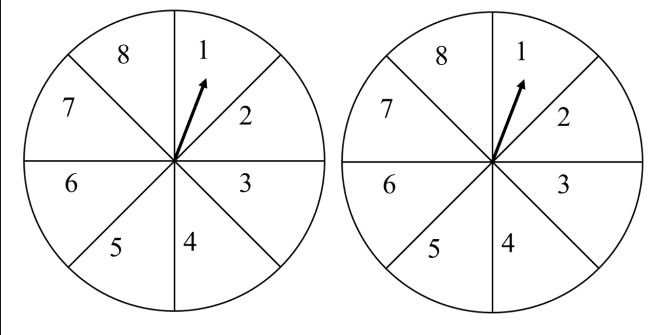
\includegraphics[width = 0.5\columnwidth]{figs/02.png}
\caption*{}
\label{fig:q7}
\end{figure}
\begin{enumerate}
\item $\frac{1}{16}$
\vspace{0.3cm}
\item $\frac{5}{64}$
\vspace{0.3cm}
\item $\frac{3}{32}$
\vspace{0.3cm}
\item $\frac{7}{64}$
\end{enumerate}

\item Consider the following inequalities.
\begin{align*}
\brak{\text{i}} \qquad 3p-q&<4\\
\brak{\text{ii}}\qquad 3q-p&<12
\end{align*}
Which one of the following expressions below satisfies the above two inequalities?

\hfill{\brak{\text{GATE GG 2022}}}
\begin{enumerate}
\item $p+q<8$
\item $p+q=8$
\item $8\le p+q<16$
\item $p+q\ge16$
\end{enumerate}

\item Given below are three statements and four conclusions drawn based on the statements.
\begin{itemize}
\item Statement 1: Some engineers are writers.
\item Statement 2: No writer is an actor.
\item Statement 3: All actors are engineers.
\end{itemize}
\begin{itemize}
\item Conclusion I: Some writers are engineers.
\item Conclusion II: All engineers are actors.
\item Conclusion III: No actor is a writer.
\item Conclusion IV: Some actors are writers.
\end{itemize}
Which one of the following options can be logically inferred?

\hfill{\brak{\text{GATE GG 2022}}}
\begin{enumerate}
\item Only conclusion I is correct
\item Only conclusion II and conclusion III are correct
\item Only conclusion I and conclusion III are correct
\item Either conclusion III or conclusion IV is correct
\end{enumerate}

\item Which one of the following sets of pieces can be assembled to form a square with a single round hole near the center? Pieces cannot overlap.

\hfill{\brak{\text{GATE GG 2022}}}
\begin{figure}[H]
\begin{enumerate}
\item \centering 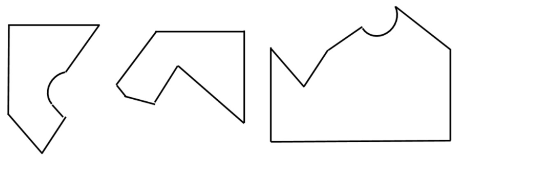
\includegraphics[width = 0.5\columnwidth]{figs/03.png} 
\item \centering 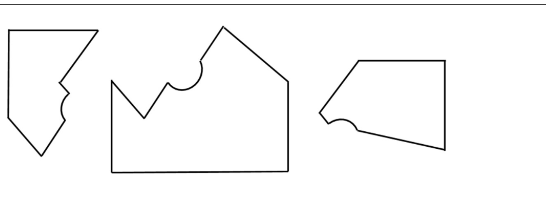
\includegraphics[width = 0.5\columnwidth]{figs/04.png}
\item \centering 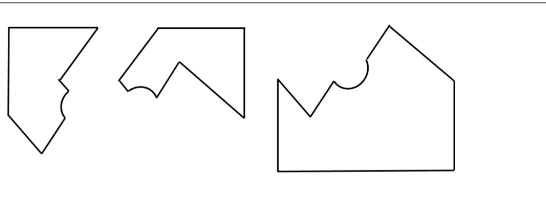
\includegraphics[width = 0.5\columnwidth]{figs/05.png}
\item \centering 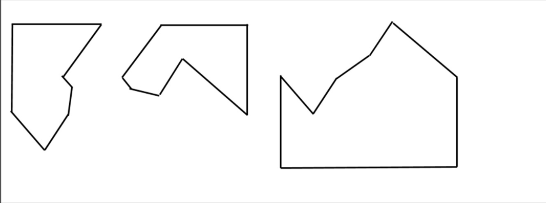
\includegraphics[width = 0.5\columnwidth]{figs/06.png}
\end{enumerate}
\caption*{}
\label{fig:q10}
\end{figure}

\item Which one of the following is the typical product of ductile deformation?

\hfill(GATE GG 2022)
\begin{enumerate}
\item Gouge
\item Breccia
\item Cataclasite
\item Mylonite
\end{enumerate}

\item Which one among the following coastal erosional landforms is caused by the action of sea waves?

\hfill(GATE GG 2022)
\begin{enumerate}
\item Ventifact
\item Kettle
\item Cirque
\item Cliff
\end{enumerate}

\item In which one of the following regions of the electromagnetic spectrum does the maximum atmospheric scattering occur?

\hfill(GATE GG 2022)
\begin{enumerate}
\item UV
\item IR
\item Radiowave
\item Microwave
\end{enumerate}

\item Which one of the following is the Poisson$'$s ratio for an incompressible fluid?

\hfill(GATE GG 2022)
\begin{enumerate}
\item $0$
\item $0.25$
\item $1$
\item $0.5$
\end{enumerate}

 \item Which among the following Period(s) belong(s) to the Paleozoic Era?

\hfill(GATE GG 2022)
\begin{enumerate}
\item Carboniferous
\item Paleogene
\item Silurian
\item Cretaceous
\end{enumerate}
\vspace{0.3cm}

\item The average bulk density of a fully saturated sandstone reservoir with a fractional porosity of $0.23$ is  \makebox[2cm]{\hrulefill} g/cc. \sbrak{\text{round off to $2$ decimal places}} \\
\sbrak{\text{Assume matrix density = $2.63$ g/cc and fluid density = $1.05$ g/cc}}
\hfill(GATE GG 2022)
\vspace{0.5cm}

\item For a productive alluvial aquifer with hydraulic conductivity = $105$ m/day and hydraulic gradient = $0.01$, the flow rate is \makebox[2cm]{\hrulefill} m/day. \sbrak{\text{round off to $2$ decimal places}}
\hfill(GATE GG 2022)
\vspace{0.5cm}

\item The relationship between conjugate shear fractures and the principal stresses 
in a homogenous, isotropic, deformed body is shown in the stereoplot 
($\sigma_1, \sigma_2, \sigma_3$ are compressive stresses).  Which one of the given fault regimes is indicated according to the Anderson$'$s theory of faulting for the formation of conjugate shear fractures under plane strain?
\hfill(GATE GG 2022)
\begin{figure}[H]
\centering
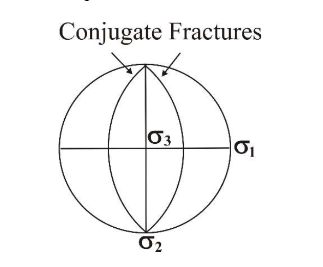
\includegraphics[width = 0.42\columnwidth]{figs/07.png}
\caption*{}
\label{fig:q5}
\end{figure}
\begin{multicols}{2}
\begin{enumerate}
\item Dextral strike-slip
\item Sinistral strike-slip
\item Reverse
\item Normal
\end{enumerate}
\end{multicols}

\item How many independent elastic parameters are needed to describe a homogenous isotropic material?

\hfill(GATE GG 2022)
\begin{enumerate}
\item $21$
\item $2$
\item $36$
\item $3$
\end{enumerate}

\item Which one of the following is a mafic volcanic rock?

\hfill(GATE GG 2022)
\begin{enumerate}
\item Dacite
\item Trachyte
\item Rhyolite
\item Basalt
\end{enumerate}

\item The intercepts of a crystal face on the crystallographic axes are $\infty a, 2b, 3c$.  
Which one of the following is its Miller Index?

\hfill(GATE GG 2022)
\begin{enumerate}
\item (032)
\item (023)
\item (203)
\item (320)
\end{enumerate}

\item Match the locations in Group I with the corresponding economic deposits in Group II.
\hfill(GATE GG 2022)
\begin{tabular}{ l l }
\textbf{Group I} & \textbf{Group Il}\\
P. Wajrakarur & 1. Chromite \\
 Q. Sukinda & 2. Diamond\\
 R. Malanjkhand &  3. Barite\\
 S. Mangampeta & 4. Copper
\end{tabular}
\begin{enumerate}
\item P-3; Q-4; R-1; S-2
\item P-3; Q-1; R-4; S-2
\item P-2; Q-1; R-4; S-3
\item P-2; Q-4; R-1; S-3
\end{enumerate}

\item Choose the CORRECT statement(s) on seismic wave propagation in an elastic isotropic medium.

\hfill(GATE GG 2022)
\begin{enumerate}
\item P-waves are polarized in the direction of propagation
\item S-waves are polarized in the direction of propagation
\item Rayleigh waves are elliptically polarized
\item Love waves are elliptically polarized
\end{enumerate}

\item The difference in arrival times of P- and S-waves generated by an earthquake and recorded at a seismological station is one second. Assuming VP = $3$ km/s and VP/VS = $2.0$, the distance between the station and the hypocenter is \makebox[2cm]{\hrulefill} km. \sbrak{\text{round off to $1$ decimal place}}
\hfill(GATE GG 2022)
\vspace{0.5cm}

\item Assuming the rate of rotation of the Earth is $7.27 \times 10^{-5}$ rad/s and the radius of Earth is $6371$ km, the centrifugal acceleration at $60\degree$ latitude is  \makebox[2cm]{\hrulefill}$\times 10^{-3}$ m/s$^2$. \sbrak{\text{round off to 1 decimal place}}
\hfill(GATE GG 2022)
\vspace{0.5cm}

\item The angle of inclination of the remanent magnetization of a volcanic rock measured at a location is 45$\degree$. The magnetic latitude of the location of the volcanic rock at the time of its magnetization is  \makebox[2cm]{\hrulefill}$\degree$N. \sbrak{\text{round off to 1 decimal place}}\\
\hspace*{15.7cm}(GATE GG 2022)
\textbf{PART B (SECTION 1):FOR GEOPHYSICS CANDIDATES ONLY}
\vspace{0.5cm}

\item In 2D stacked seismic sections, the vertical axis corresponds to two-way travel time and the horizontal axis corresponds to\makebox[2cm]{\hrulefill} . 

\hfill(GATE GG 2022)
\begin{enumerate}
\item receiver locations  
\item source locations  
\item Offsets  
\item common midpoint (CMP) locations  
\end{enumerate}

\item In a 2D seismic survey acquired on land, head waves were recorded at the surface. Assuming that the subsurface consisted of horizontal, isotropic and homogeneous layers, the moveout of the head wave event(s) would be  \makebox[2cm]{\hrulefill} . 

\hfill(GATE GG 2022)
\begin{enumerate}
\item linear  
\item parabolic  
\item hyperbolic  
\item elliptical  
\end{enumerate}


\item An accurate depth migration of seismic data requires the knowledge of \makebox[2cm]{\hrulefill} .

\hfill(GATE GG 2022)
\begin{enumerate}
\item interval velocities  
\item root mean squared (RMS) velocities  
\item stacking velocities  
\item normal moveout (NMO) velocities  
\end{enumerate}

\item The dimension of bulk modulus is  \makebox[2cm]{\hrulefill} .

\hfill(GATE GG 2022)
\begin{enumerate}
\item $[M L^{-1} T^{-2}]$  
\item $[M L T^{-2}]$  
\item $[M L^{-2} T^{-2}]$  
\item $[M L^{2} T^{-2}]$  
\end{enumerate}

\item A current flows from a medium with resistivity $\rho_1$ to a medium with resistivity $\rho_2$. A planar interface separates the two media. The angle of incidence and refraction with respect to the normal to the interface are $\theta_1$ and $\theta_2$, respectively. If the components of the current density perpendicular to the interface and the components of the electric field horizontal to the interface are continuous, the electrical law of refraction can be expressed as \makebox[2cm]{\hrulefill} .

\hfill(GATE GG 2022)
\begin{enumerate}
\item $\rho_1 \tan \theta_1 = \rho_2 \tan \theta_2$  
\item $\rho_1 \sin \theta_1 = \rho_2 \sin \theta_2$  
\item $\rho_2 \cos \theta_1 = \rho_1 \cos \theta_2$  
\item $\rho_1 \tan \theta_2 = \rho_2 \tan \theta_1$  
\end{enumerate}

\item The convolution of two box-car pulses of positive amplitudes, with unequal and finite durations yields a \makebox[2cm]{\hrulefill}pulse.  

\hfill(GATE GG 2022)
\begin{enumerate}
\item triangular  
\item trapezoidal  
\item rectangular  
\item sinusoidal  
\end{enumerate}


\item Which ONE of the following P-phases represents a reflection from the Moho?  
\hfill(GATE GG 2022)
\begin{enumerate}
\item Pn  
\item Pg  
\item P*  
\item PmP  
\end{enumerate}


\item The remanent, induced and total magnetizations of a rock sample are denoted by $\vec{M_r}$, $\vec{M_i}$ and $\vec{M_t}$, respectively. The Konigsberger ratio is  

\hfill(GATE GG 2022)
\begin{enumerate}
\item $\dfrac{|\vec{M_i}|}{|\vec{M_t}|}$  
\item $\dfrac{|\vec{M_r}|}{|\vec{M_t}|}$  
\item $\dfrac{|\vec{M_t}|}{|\vec{M_i}|}$  
\item $\dfrac{|\vec{M_t}|}{|\vec{M_r}|}$  
\end{enumerate}


\item Which among the following is/are CORRECT statement(s) about the Van Allen radiation belts?  

\hfill(GATE GG 2022)
\begin{enumerate}
\item The inner belt consists mainly of protons and the belt extends to about $1000-3000$ km from the Earth$'$s surface.  
\item The belts are doughnut-shaped regions coaxial with the geomagnetic field lines of the Earth.  
\item The pitch of the helical motion of the charged particles increases as the particles approach the surface of the Earth.  
\item The outer belt occupies regions between 3 to 4 Earth radii and consists primarily of electrons.  
\end{enumerate}


\item Which of the following logging methods can be used to measure the resistivity of the flushed zone?  

\hfill(GATE GG 2022)
\begin{enumerate}
\item Lateral log  
\item Long normal log  
\item Microlaterolog  
\item Microspherically focused log  
\end{enumerate}

\item Which of the following statement(s) is/are CORRECT about the continuation of the gravity field?  

\hfill(GATE GG 2022)
\begin{enumerate}
\item Continuation of the gravity field from one surface to another is permissible only when there are no masses present between the two surfaces.  
\item In upward continuation, the longer wavelength anomalies are attenuated more than the shorter wavelength anomalies.  
\item Downward continuation may enhance noise and uncertainties.  
\item Upward continuation is a smoothing process.  
\end{enumerate}

\item An oceanic plate formed at a mid-oceanic ridge $27$ million years ago. The plate has been moving with a uniform half-spreading rate of $4$ cm/year ever since its formation. The current distance between the edge of this plate and the centre of the ridge is \makebox[2cm]{\hrulefill} km.\sbrak{\text{round  off to 1 decimal place}}
\hfill(GATE GG 2022)
\vspace{0.5cm}

\item
An artificial neural network \brak{\text{ANN}} is trained to classify between shale and sand formations. The final layer of the ANN consists of a single neuron with a sigmoid activation function given by  $\sigma(x) = \frac{1}{1+e^{-x}}$If the input to the final neuron is 0, then the output is \makebox[2cm]{\hrulefill}. \sbrak{\text{round off to 1 decimal place}}  
\hfill(GATE GG 2022)
\vspace{0.5cm}

\item A current electrode introduces a $2$ Ampere current at a point \brak{P} on  the surface of a uniform half space. If the resistivity of the half space is $5$ $\Omega$-m, the magnitude of the electric field (due to the current) in the half space at a distance of $1$ m from P is \makebox[2cm]{\hrulefill} V/m. \sbrak{\text{round off to 2 decimal places}}
\hfill(GATE GG 2022)
\vspace{0.5cm}
  
\item The relative dielectric permittivity of a homogeneous isotropic medium is 10 and the relative magnetic permeability of the same medium is 1. If the velocity of the electromagnetic wave propagating through this medium is $v$ and the velocity of light in vacuum is $c$, then the ratio $v/c$ is \makebox[2cm]{\hrulefill} V/m. \sbrak{\text{round off to 2 decimal places}}
\hfill(GATE GG 2022)
\vspace{0.5cm}

\item A mountain of height 8 km above mean sea level is in isostatic equilibrium with a 42 km thick continental crust. As predicted by Airy$'$s hypothesis, the root beneath this mountain is \makebox[2cm]{\hrulefill} V/m. \sbrak{\text{round off to 2 decimal places}}  

\sbrak{\text{Assume: density of mantle = $3.7 \times 10^3 \,\text{kg m}^{-3}$ and density of crust = $2.7 \times 10^3 \,\text{kg m}^{-3}$}}
\hfill(GATE GG 2022)
\vspace{0.5cm}

\item In wet soil of resistivity 100 $\Omega$m, the skin depth of a GPR signal of 100 MHz is \makebox[2cm]{\hrulefill} V/m. \sbrak{\text{round off to 2 decimal places}}  
\sbrak{\text{Assume: $\mu_0 = 4 \pi \times 10^{-7} \, H/m$}}
\hfill(GATE GG 2022)
\vspace{0.5cm}


\item A Wadati diagram was prepared for a local earthquake occurring in a homogeneous crust. If the crust is assumed to be a Poisson solid, the slope of the straight line in the Wadati diagram is \makebox[2cm]{\hrulefill} V/m. \sbrak{\text{round off to 2 decimal places}}
\hfill(GATE GG 2022)
\vspace{0.5cm}

\item The gravitational potential of the spheroidal Earth can be expressed as    \textbf{$U = -\dfrac{G M}{r}\left[1 - \sum_{n=2}^{\infty} \left(\dfrac{R}{r}\right)^n J_n P_n(\cos \theta)\right],$}
where $G$ is the gravitational constant, $M$ is the mass of the Earth, $r$ is the radial distance from the centre of the Earth, $R$ is the radius of Earth, $J_n$ are coefficients obtained from satellite geodesy, $P_n$ represents the Legendre polynomial of order $n$, and $\theta$ is the colatitude.  
Which among the following is described by the term corresponding to $n=2$?\\  
\sbrak{\text{Given: $P_2(\cos \theta) = \tfrac{1}{2}(3 \cos^2\theta -1)$}}  
\hfill(GATE GG 2022)

\begin{enumerate}
\item Gravitational potential due to a spherical Earth  
\item Deviations from the ellipsoid that correspond to a pear-shaped Earth  
\item The effect of the polar flattening on the Earth$'$s gravitational potential  
\item The gravitational potential of the Earth-Moon system  
\end{enumerate}

\item The magnetic potential of a dipole at any external point (P) can be expressed as  $V = C_1 \, \frac{\vec{m}\cdot \hat{r}}{r^2}, \quad r \neq 0,$
where $\vec{m}$ is the dipole moment, $\hat{r}$ is a unit normal along the vector directed from the centre of the dipole to the external point (P) and $C_1$ is a constant.  If $\theta$ is the angle between $\vec{m}$ and $\hat{r}$, the radial component of $\vec{B}$ is:  

\hfill(GATE GG 2022)
\begin{enumerate}
\item $B_r = \dfrac{2 C_1 m \cos\theta}{r^3}$  
\item $B_r = \dfrac{C_1 m \cos\theta}{r^2}$  
\item $B_r = \dfrac{C_1 m \cos\theta}{r^3}$  
\item $B_r = \dfrac{2 C_1 m \cos\theta}{r^2}$  
\end{enumerate}

\item The functions $g(t)$ and $G(\omega)$ constitute a Fourier Transform pair [$g(t) \leftrightarrow G(\omega)$] as per the convention:  
$g(t) = \frac{1}{2\pi} \int_{-\infty}^{\infty} G(\omega) e^{j \omega t} d\omega, \text{and}  G(\omega) = \int_{-\infty}^{\infty} g(t) e^{-j \omega t} \, dt
$Which ONE among the following is the correct Fourier transform pair?  

\hfill(GATE GG 2022)
\begin{enumerate}
\item $\dfrac{d g(t)}{dt} \leftrightarrow G(\omega)$  
\item $\dfrac{d g(t)}{dt} \leftrightarrow j \omega G(\omega)$  
\item $\dfrac{d g(t)}{dt} \leftrightarrow -j \omega G(\omega)$  
\item $\dfrac{d g(t)}{dt} \leftrightarrow \omega G(\omega)$  
\end{enumerate}

\item Gauss divergence theorem is given by  
$\int_V \nabla \cdot \vec{a} \, dV = \int_S \vec{a} \cdot d\vec{S},
$ where $\vec{a}$ is a vector field and $V$ is the volume enclosed by the surface $S$.  If $\vec{a} = \nabla \phi + \nabla \times \vec{\psi}$, then the application of divergence theorem to $\vec{a}$ yields:  

\hfill(GATE GG 2022)
\begin{enumerate}
\item $\int_V \nabla^2 \phi \, dV = \int_S \nabla \phi \cdot d\vec{S}$  
\item $\int_V \nabla \cdot \vec{\psi} \, dV = \int_S \vec{\psi} \cdot d\vec{S}$  
\item $\int_V \nabla^2 \phi \, dV = \int_S \big(\nabla \times \vec{\psi}\big)\cdot d\vec{S}$  
\item $\int_V \phi \, dV = \int_S \vec{\psi}\cdot d\vec{S}$  
\end{enumerate}

\item The angular frequency ($\omega$) and wavenumber ($k$) for an electromagnetic wave is related by the expression  
$\omega^2 = \alpha k + \beta k^2,$ where $\alpha$ and $\beta$ are constants.  
The wavenumber $k_0$ for which the group velocity equals the phase velocity is \makebox[2cm]{\hrulefill}.  

\hfill(GATE GG 2022)
\begin{enumerate}
\item $3\sqrt{\frac{\alpha}{\beta}}$  
\item $\frac{1}{3}\sqrt{\frac{\alpha}{\beta}}$  
\item $\sqrt{\frac{\alpha}{\beta}}$  
\item $\frac{1}{2}\sqrt{\frac{\alpha}{\beta}}$  
\end{enumerate}

\item The schematic represents P-wave arrivals from a zero-offset Vertical Seismic Profiling (VSP) experiment conducted over a horizontally layered and isotropic Earth. Match the four events labelled in the schematic and their listed descriptions.  
\begin{figure}[H]
\centering
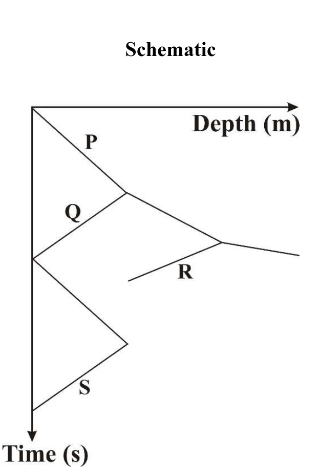
\includegraphics[width = 0.19\columnwidth]{figs/16.png}
\caption*{}
\label{fig:q5}
\end{figure}
\begin{tabular}{ l l }

\textbf{label} & \textbf{Description} \\
P & Primary reflection from the first reflector \\
Q & Direct arrival \\
R & First order multiple \\
S & Primary reflection from the second reflector \\
\end{tabular}

\hfill(GATE GG 2022)
\begin{enumerate}
\item P-2; Q-1; R-4; S-3  
\item P-1; Q-2; R-3; S-4  
\item P-2; Q-1; R-3; S-4  
\item P-1; Q-2; R-4; S-3  
\end{enumerate}

\item The transfer function of a linear system is given as  $H(s) = \frac{s+2}{s^2+5s+6}$.The poles of this function are   \makebox[2cm]{\hrulefill}

\hfill(GATE GG 2022)
\begin{enumerate}
\item $-3$ and $-2$  
\item $-3$ and $2$  
\item $3$ and $-2$  
\item $3$ and $2$  
\end{enumerate}

\item The eigenvalues of the given matrix $A$ are.  
$A = \begin{bmatrix}
2 & -1 & 1 \\
-1 & 0 & 1 \\
1 & 1 & 2
\end{bmatrix}$

\hfill(GATE GG 2022)
\begin{enumerate}
\item $-1$, $2$ and $3$  
\item $1$, $2$ and $3$  
\item $0$, $2$ and $3$  
\item $0$, $2$ and $2$  
\end{enumerate}

\item  The apparent resistivity values obtained from a vertical electrical sounding (VES) survey over a horizontally layered 1-D Earth are indicated by $\rho_1, \rho_2, \rho_3, \rho_4$. Match the VES curve types in Group-I with the corresponding ordering of resistivity values in Group-II.  
\hfill(GATE GG 2022)\\

\begin{tabular}{l l}
\textbf{Group-I} &\textbf{Group-II}  \\ 
P. QH & 1. $\rho_1 < \rho_2 > \rho_3 < \rho_4$ \\ 
Q. HK & 2. $\rho_1 > \rho_2 > \rho_3 < \rho_4$ \\ 
R. HA & 3. $\rho_1 > \rho_2 < \rho_3 > \rho_4$ \\ 
S. KH & 4. $\rho_1 > \rho_2 < \rho_3 < \rho_4$ \\ \
\end{tabular}

\begin{enumerate}
\item P-4; Q-3; R-1; S-2  
\item P-2; Q-3; R-4; S-1  
\item P-4; Q-3; R-2; S-1  
\item P-3; Q-1; R-2; S-4  
\end{enumerate}

\item Choose the CORRECT statement(s) from the following on the solution of systems of linear equations without the application of regularization.  

\hfill(GATE GG 2022)
\begin{enumerate}
\item An under-determined system of linearly independent equations has either a trivial solution or an infinite number of solutions.  
\item An ill-conditioned system of linear equations can yield stable solutions in the presence of noise.  
\item An over-determined system of linearly independent equations does not have an exact solution.  
\item A system of linearly independent equations with the number of equations equal to the number of unknowns is a mixed-determined system.  
\end{enumerate}

\item In seismic spiking deconvolution with an unknown source wavelet, the wavelet can be deconvolved most effectively under which of the following condition(s)?

\hfill(GATE GG 2022)
\begin{enumerate}
\item The source wavelet is minimum phase.  
\item The source wavelet is zero phase.  
\item The autocorrelation of the reflectivity series in time domain can be approximated by a delta function.  
\item The autocorrelation of the reflectivity series in time domain can be approximated to be identically zero.  
\end{enumerate}

\item  The stacking chart for an end-on 2D seismic survey is shown in the figure. The shot, receiver, mid-point and offset coordinate axes are as indicated in the figure, while each star represents a unique seismic trace. With reference to the stacking chart, which of the following is/are CORRECT statement(s)? 
\hfill(GATE GG 2022)
\begin{figure}[H]
\centering
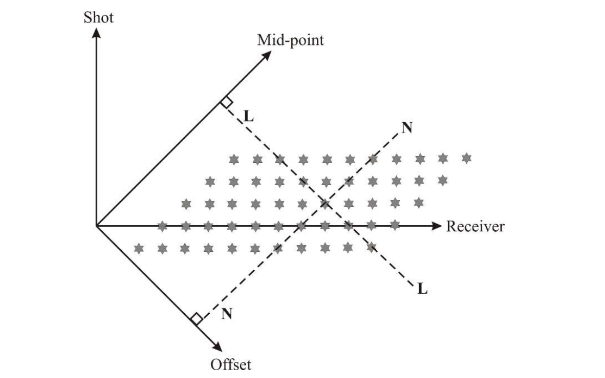
\includegraphics[width = 0.5\columnwidth]{figs/17.png}
\caption*{}
\label{fig:q5}
\end{figure}
\begin{enumerate}
\item The traces along LL constitute a common mid-point (CMP) gather.  
\item The traces along LL constitute a common shot gather.  
\item The traces along NN constitute a common offset gather.  
\item The traces along NN constitute a common receiver gather.  
\end{enumerate}

 \item Suppose $x_\frac{1}{5}$ defines the half-width at 1/5th of the maximum gravity value measured over a buried sphere of uniform density. If $d$ is the distance from the surface to the centre of the sphere, the value of $
 \frac{x_\frac{1}{5}}{d}$ is \makebox[2cm]{\hrulefill}. \sbrak{\text{round off to 2 decimal places}} 
 \hspace*{15.7cm}(GATE GG 2022)
\vspace{0.5cm}

\item In a reservoir zone, the deep induction log reads $3$ $\Omega$m for a formation whose porosity is $19$\%.  The hydrocarbon saturation of that formation from Archie$'$s equation is \makebox[2cm]{\hrulefill}\%.\sbrak{\text{round off to 1 decimal place}}
\sbrak{\text{Assume $a=1$, $m=1.5$, $n=2$, $R_w = 0.04\,\Omega$m}}
\hfill(GATE GG 2022)
\vspace{0.5cm}

\item The heat flow $q$ (mW/m$^2$) is related to the age $t$ (My) of ocean floor as $t=(510/q)^2$.  At a site in the Indian Ocean, geothermal gradient = $55^\degree$C/km, $k=2.3$ W/m$\cdot^\degree$C. The site age is \makebox[2cm]{\hrulefill} My. \sbrak{\text{round off to 2 decimal places}} 
\hfill(GATE GG 2022)
\vspace{0.5cm}

\item The isotopes $A_X$ and $B_X$ of an element $X$ were initially equal in abundance. Later, the observed ratio was $B_X/A_X = 128.55$.  
The elapsed time since formation =\makebox[2cm]{\hrulefill}  years.\sbrak{\text{round off to 1 decimal place}}  
[$\lambda_A = 9.85 \times 10^{-3} \, y^{-1}$, $\lambda_B = 1.55 \times 10^{-3} \, y^{-1}$]  
\hfill(GATE GG 2022)
\vspace{0.5cm}

\item A two-layer planet \brak{\text{core + mantle}}. Core density = $7150$ kg/m$^3$,  
planet mean density = $5620$ kg/m$^3$. Mantle extends over outer $2/3$ of radius.  Density of mantle = \makebox[2cm]{\hrulefill} kg/m$^3$. \sbrak{\text{round off to 1 decimal place}}  
\hfill(GATE GG 2022)
\vspace{0.5cm}

\item A reflection seismic survey is conducted over a two-layered medium with a single horizontal, homogeneous, isotropic layer underlain by a homogenous,isotropic half-space. The Shuey two-term approximation for the P-wave reflection coefficient for the interface separating the media is given by:  
$R(\theta) = 0.025 - 0.1 \sin^2 \theta,$
where $\theta$ is the angle of incidence of the P-wave with respect to the normal to the interface. Assuming the validity of the approximation, the offset-to-depth ratio (offset/depth) at which a polarity reversal can be observed in a CMP gather from the survey is \makebox[2cm]{\hrulefill}. \sbrak{\text{round off to 1 decimal place}}  
\text{[Hint: A change in the sign of the reflection coefficient leads to polarity reversal]} 
\hfill(GATE GG 2022)
\vspace{0.5cm}


\item The given figure shows the rupture of a unilateral fault with the rupture velocity ($V_r$) of $2$ km/s. According to the simple Haskell source model, the rupture time associated with the entire length of the fault as estimated at the station is \makebox[2cm]{\hrulefill} sec. \sbrak{\text{round off to 2 decimal places}}
\text{[Assume: Shear wave speed = 3.5 km/s]}
\hfill(GATE GG 2022)
\begin{figure}[H]
\centering
	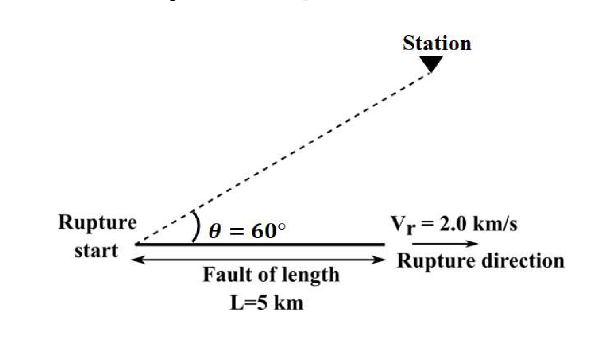
\includegraphics[width = 0.4\columnwidth]{figs/18.png}
\caption*{}
\label{fig:q5}
\end{figure}
  
\vspace{0.5cm}

\item The given figure shows ray paths for direct P and P-to-S converted phases 
recorded at a station on the surface (R) for a teleseismic event. Given that the 
ray parameter ($p$) is $0.1 \, \text{s/km}$, the arrival time difference between 
the P-to-S converted phase and the direct P-phase at the receiver R is  \makebox[2cm]{\hrulefill} sec. \sbrak{\text{round off to 2 decimal places}}
\hfill(GATE GG 2022)
\begin{figure}[H]
\centering
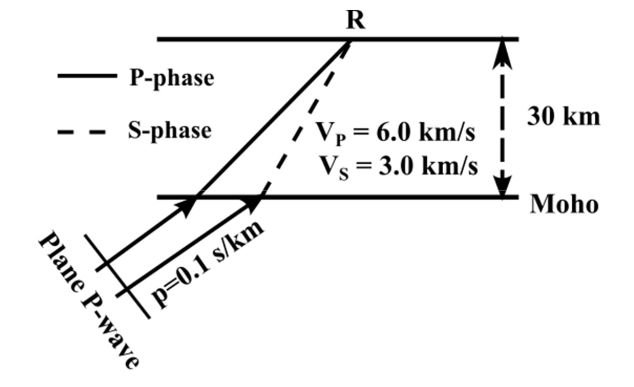
\includegraphics[width = 0.5\columnwidth]{figs/19.png}
\caption*{}
\label{fig:q5}
\end{figure}
\vspace{0.5cm}

\item A land seismic survey is conducted over a horizontally layered and isotropic Earth. The thickness and the P-wave velocity of the homogeneous weathered layer are $5$ m and $800$ m/s, respectively. The shots are fired at a depth of $5$ m below the surface and the receivers are placed on the surface at mean sea level \brak{MSL}. If the datum plane is defined to be $5$ m below the MSL, the magnitude of the P-wave static correction to be applied to the data is \makebox[2cm]{\hrulefill} milli sec. \sbrak{\text{round off to 2 decimal places}} 
\hspace*{15.7cm}(GATE GG 2022)

\end{enumerate}
\end{document}
